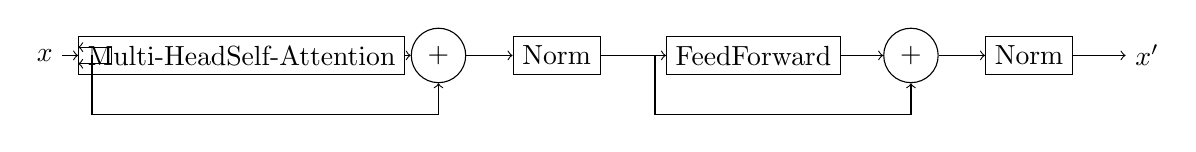
\begin{tikzpicture}[]
        %% Nodes
        \node[rectangle, draw] (mhsa) at (2.5,0)  {Multi-Head\\Self-Attention};
        \node[circle, draw] (sum1) at (5, 0) {$+$};
        \node[rectangle, draw] (norm1) at (6.5,0) {Norm};
        
        \node[rectangle, draw] (ffwd) at (9,0) {Feed\\Forward};
        \node[circle, draw] (sum2) at (11,0) {$+$};
        \node[rectangle, draw] (norm2) at (12.5,0){Norm};

        \node(input) at (0, 0) {$x$};
        \node(output) at (14, 0) {$x'$};
        \node(emptres) at (0.6, 0) {};
        \node(emptres2) at (7.75, 0) {};
        \node(empt0) at (0.85, 0) {};
        \node(empt1) at (2.75, -.75) {};
        \node(empt2) at (10, -.75) {};
        
        
        %% Edges
        \draw[->] (input.east) -- node {} (mhsa.west);
        \draw[->] (empt0.center) |- node {} ([yshift=-4pt] mhsa.north west);
        \draw[->] (empt0.center) |- node {} ([yshift= 4pt] mhsa.south west);
        \draw[-] (emptres.center) |- node {} (empt1.center);
        \draw[->] (empt1.center) -| node {} (sum1.south);
        \draw[->] (mhsa.east) -- node {} (sum1.west);
        \draw[->] (sum1.east) -- node {} (norm1.west);

        \draw[->] (norm1.east) -- node {} (ffwd.west);
        \draw[-] (norm1.east) -- node {} (emptres2.center);
        \draw[-] (emptres2.center) |- node {} (empt2.center);
        \draw[->] (empt2.center) -| node {} (sum2.south);
        \draw[->] (ffwd.east) -- node {} (sum2.west);
        \draw[->] (sum2.east) -- node {} (norm2.west);
        \draw[->] (norm2.east) -- node {} (output.west);
\end{tikzpicture}    